\begin{titlepage}
\begin{center}

{\small Київський національний університет  імені Тараса Шевченка}

{\small фізичний факультет}


\vspace*{2cm}
{\scshape\bfseries\Large О.Я.~ОЛІХ}

\vspace*{1cm}
{\scshape\bfseries\huge методи дослідження дефектів}

\vspace*{0.5cm}
методичний посібник для студентів фізичного факультету

\end{center}
%
\vspace*{2cm}
\begin{figure}[h]\center
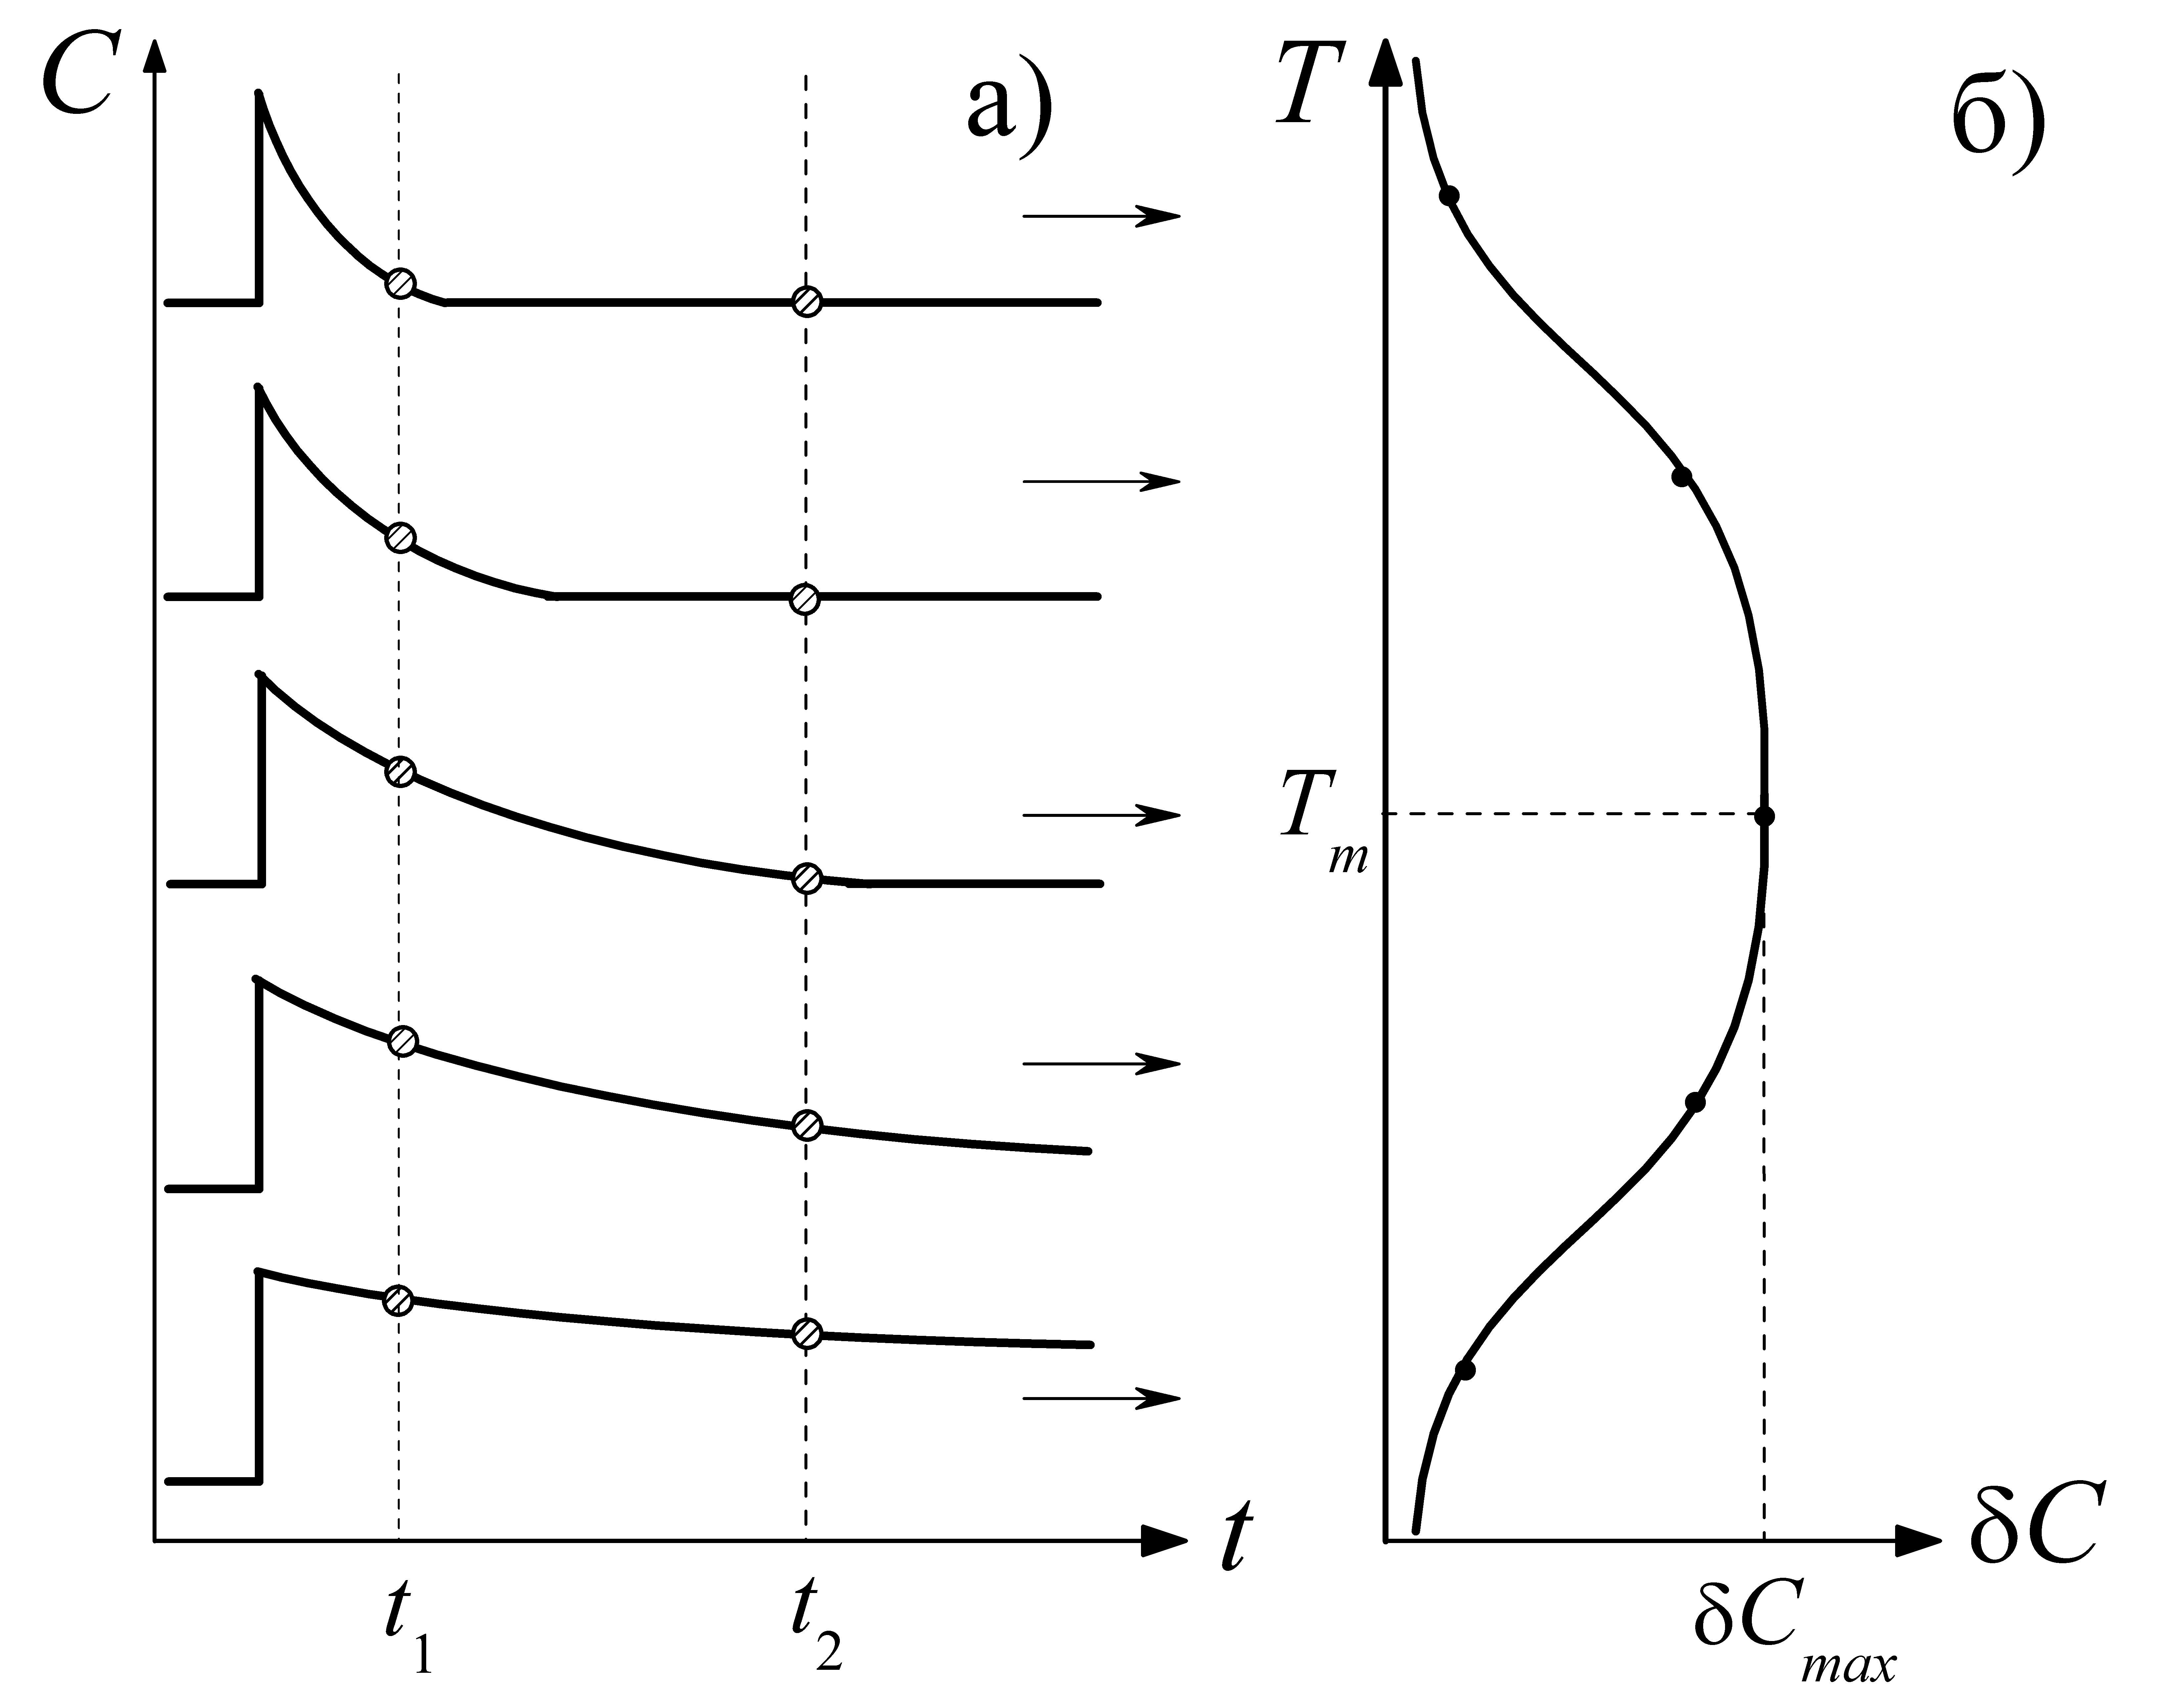
\includegraphics[width=0.8\textwidth]{Fig2_3}
\end{figure}
%
%
\begin{center}

{\scshape\bfseries Київ -- 2020}
\end{center}
\end{titlepage}
Б

УДК 004.7; 004.057.4.

\begin{center}

 \vspace{0.04\textheight}
 Рецензенти:
\end{center}
%\vspace{0.5cm}

\emph{С.В.~Кондратенко}, д-р. фіз.-мат. н., проф.

\emph{О.О.~Коротченков}, д-р. фіз.-мат. н., проф.

\vspace{1cm}
Рекомендовано до друку вченою радою фізичного факультету
Київського національного університету імені Тараса Шевченка
(протокол №10 від 18 квітня 2020 року)



\vspace{1cm}
\textbf{Оліх О.Я.}

Методи дослідження дефектів. Методичний посібник для студентів фізичного факультету. --- К.:2020.
%Іл.~236, табл.~51.

\vspace{1cm}
У посібнику розглянуто основні типи точкових дефектів, методи їх опису та термодинамічні підходи оцінки рівноважної концентрації.
Докладно викладено питання, які стосуються механізмів дифузії точкових дефектів.
Проаналізовано шляхи впливу на дефектну підсистему кристалів радіаційного опромінення і термічної обробки.
Наведено приклади найпоширеніших точкових комплексів у кремнії, а також розглянуто особливості метастабільних та бістабільних дефектів і центрів з від’ємною кореляційною енергією. Посібник містить задачі для самостійного розв’язання.
